\section{Swarm Controller Design}

As a sample swarm controller design I had choosen to implement a standard determinist swarm controller. That type of controller is following a given set of rules which are always predicable in a term of behaviour and trajectory of a drone. Good exaple of such a controller, one of the first ever described, is a Boids algorithm created by Craig Reynolds in 1986~\cite{wiki:boids}. The main idea of this algorithm is to create a swarm behaviour based on three simple rules: separation, alignment and cohesion. Separation rule is responsible for avoiding collisions between drones, alignment rule is responsible for keeping the same direction of movement as the other drones in the swarm and cohesion rule is responsible for keeping the swarm together.
 This is opossite of controller based on a neural network or genetic algorithm where set of rules is being created in a training process. Nevertheless neural network controller or any other different kind could be tested in this simulator as well. 




 \subsection{Data Fusion, KF and Localization}
    In order to create a swarm controller that is able to control multiple drones at the same time, it is necessary to have a precise localization of drones in both global frame and local, drones, frame. For that purpose I have used Kalman Filter (KF) to fuse data from GPS, IMU, compass and LoRa ToF. 

    One major achievement of this system is that even if one of the drones in the swarm is not able to receive GPS signal, it is still able to localize itself based on the data from other drones in the swarm. This is possible thanks to the fact that each drone is equipped with a LoRa ToF sensor that is able to measure the distance to other drones in the swarm. By fusing data it is possible to create a precise localization of each drone in the swarm even if one of them is not able to receive GPS signal. Or a GPS signal is being jammed or spoofed.



    \subsection{KF State Space and Filter Design}

    The Kalman Filter implemented for this project operates on a
    four-dimensional state vector consisting of geographic position and
    horizontal velocity:

    \begin{equation}
        \mathbf{x} = \begin{bmatrix} \phi \\ \lambda \\ v_x \\ v_z \end{bmatrix}
    \end{equation}

    where $\phi$ is latitude (degrees), $\lambda$ is longitude (degrees),
    $v_x$ is east velocity (m/s), and $v_z$ is north velocity (m/s).
    To avoid numerical ill-conditioning from mixing angular and metric units,
    all covariance matrices are maintained internally in metres, with
    conversion applied only at the input/output boundary using the
    WGS84-derived constants:

    \begin{equation}
        k_{lat} = 111{,}111 \ \text{m/deg}, \qquad
        k_{lon} = 64{,}528 \ \text{m/deg} \quad (\text{at } 54°\text{N, Baltic Sea})
    \end{equation}

    \subsubsection{Process Model}

    The state transition is driven by a constant-velocity model augmented
    with optional IMU acceleration input. When IMU data is available,
    body-frame accelerations $(a_x^b, a_z^b)$ are first rotated into the
    world frame using the current compass heading $\psi$:

    \begin{equation}
        \begin{bmatrix} a_x^w \\ a_z^w \end{bmatrix}
        =
        \begin{bmatrix}
            \cos\psi & -\sin\psi \\
            \sin\psi &  \cos\psi
        \end{bmatrix}
        \begin{bmatrix} a_x^b \\ a_z^b \end{bmatrix}
    \end{equation}

    To prevent unbounded IMU drift in the absence of GPS corrections,
    an exponential velocity decay with a 3-second time constant is applied:

    \begin{equation}
        \alpha = e^{-\Delta t / 3}
    \end{equation}

    The discrete-time state prediction is then:

    \begin{equation}
        v_x^- = \alpha \, v_x + a_x^w \, \Delta t, \qquad
        v_z^- = \alpha \, v_z + a_z^w \, \Delta t
    \end{equation}

    \begin{equation}
        \phi^-  = \phi  + \frac{v_z^- \, \Delta t}{k_{lat}}, \qquad
        \lambda^- = \lambda + \frac{v_x^- \, \Delta t}{k_{lon}}
    \end{equation}

    The covariance prediction follows $\mathbf{P}^- = \mathbf{F}\mathbf{P}\mathbf{F}^\top + \mathbf{Q}$,
    where the linearised state transition matrix $\mathbf{F}$ captures the
    position--velocity coupling ($\delta\phi / \delta v_z = \Delta t$) and
    the velocity decay ($\delta v / \delta v = \alpha$). The process noise
    matrix $\mathbf{Q}$ is diagonal:

    \begin{equation}
        \mathbf{Q} = \operatorname{diag}(Q_{pos},\ Q_{pos},\ Q_{vel},\ Q_{vel})
    \end{equation}

    with $Q_{pos} = 0.5\ \text{m}^2/\text{tick}$ and
    $Q_{vel} = 0.5\ \text{(m/s)}^2/\text{tick}$, tuned empirically to
    balance GPS trust against IMU responsiveness.

    \subsubsection{Measurement Models}

    Three independent measurement updates are applied sequentially using
    scalar Kalman updates, which avoids matrix inversion and is numerically
    robust for embedded deployment.

    \paragraph{GPS Update.}
    The GPS measurement model is:
    \begin{equation}
        \mathbf{H}_{GPS} = \begin{bmatrix} 1 & 0 & 0 & 0 \\ 0 & 1 & 0 & 0 \end{bmatrix}
    \end{equation}

    The measurement noise variance is derived from the reported GPS accuracy:
    \begin{equation}
        R_{GPS} =
        \begin{cases}
            \sigma_{GPS}^2 & \text{if } \sigma_{GPS} > 0.5\ \text{m} \\
            25\ \text{m}^2 & \text{otherwise (conservative default)}
        \end{cases}
    \end{equation}

    Innovations are computed in metres to maintain numerical consistency:
    \begin{equation}
        \tilde{y}_{lat} = (\phi_{GPS} - \phi^-) \cdot k_{lat}, \qquad
        \tilde{y}_{lon} = (\lambda_{GPS} - \lambda^-) \cdot k_{lon}
    \end{equation}

    Kalman gains and state updates are then applied independently for each
    axis, with the position--velocity cross-covariance terms propagating
    the correction into the velocity states.

    \paragraph{Speed and Heading Update.}
    When a compass heading $\psi$ and speed $s$ are available, the
    velocity measurement is:
    \begin{equation}
        v_x^{meas} = s \sin\psi, \qquad v_z^{meas} = s \cos\psi
    \end{equation}

    with measurement noise $R_v = 0.25\ \text{(m/s)}^2$ (corresponding to
    $\sigma = 0.5\ \text{m/s}$). This update directly corrects the velocity
    states and, through the cross-covariance terms, also refines the
    position estimate.



\subsection{KF tests and validation}

    To validate the KF implementation, I have created a multiple tests in the simulator. First test was to check if the KF is able to estimate the position of the drone based on the data from GPS, IMU, compass and LoRa ToF. That position is compared to the true position of the drone in the simulator, and a GPS position from simulator. The results of the test are shown on the figure \ref{fig:KF_test_normal}. Each test was run for 5 minutes of simulation time.


    \begin{figure}[H]
        \centering
        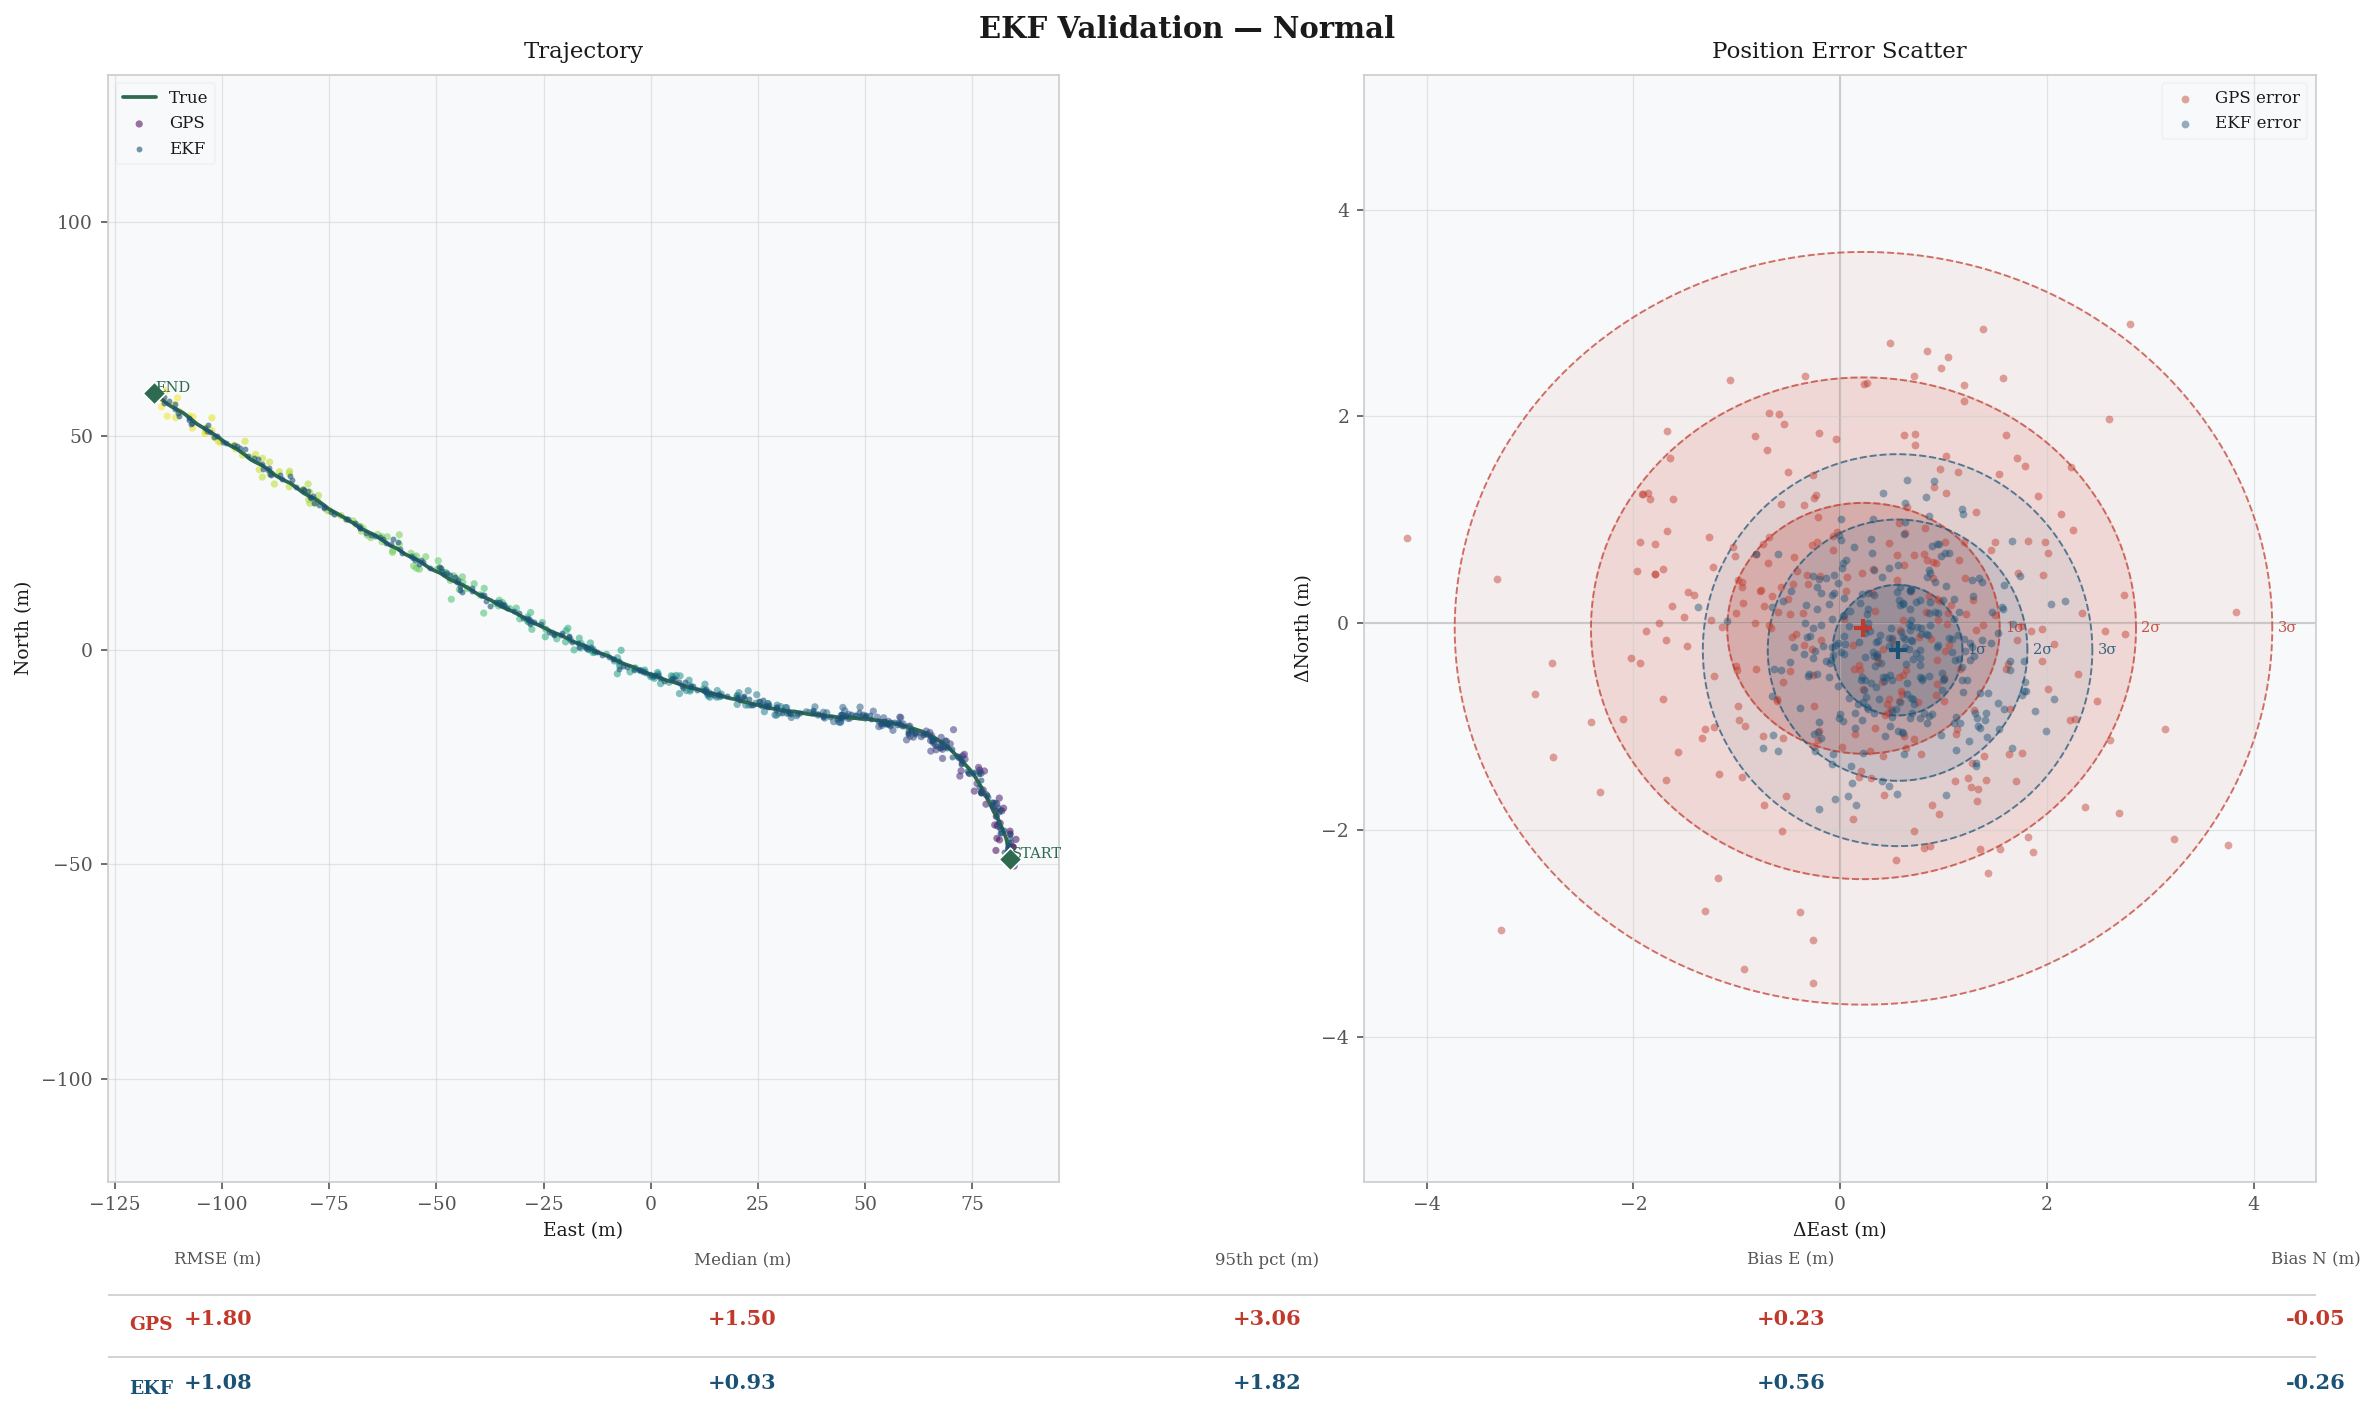
\includegraphics[width=0.9\textwidth]{images/ekf_validation_plot_normal.png}
        \caption{KF test results for normal operation. GPS RMSE is around 1.8 meters, while KF RMSE is around 1.08 meters. RED dots represent GPS position, BLUE dots represent KF position.}
        \label{fig:KF_test_normal}
    \end{figure}



    Second test was ment to check if the KF is able to estimate the position of the drone even if tested drone GPS signal is being spoofed. In this test, the GPS signal of the tested drone was being spoofed with a random noise with a standard deviation of 70 meters. The results of the test are shown on the figure \ref{fig:KF_test_gps_spoofing}. As we can see, even if the GPS signal is being spoofed, KF is still able to estimate the position of the drone with a good accuracy, with RMSE around 19 meters. 


    \begin{figure}[H]
        \centering
        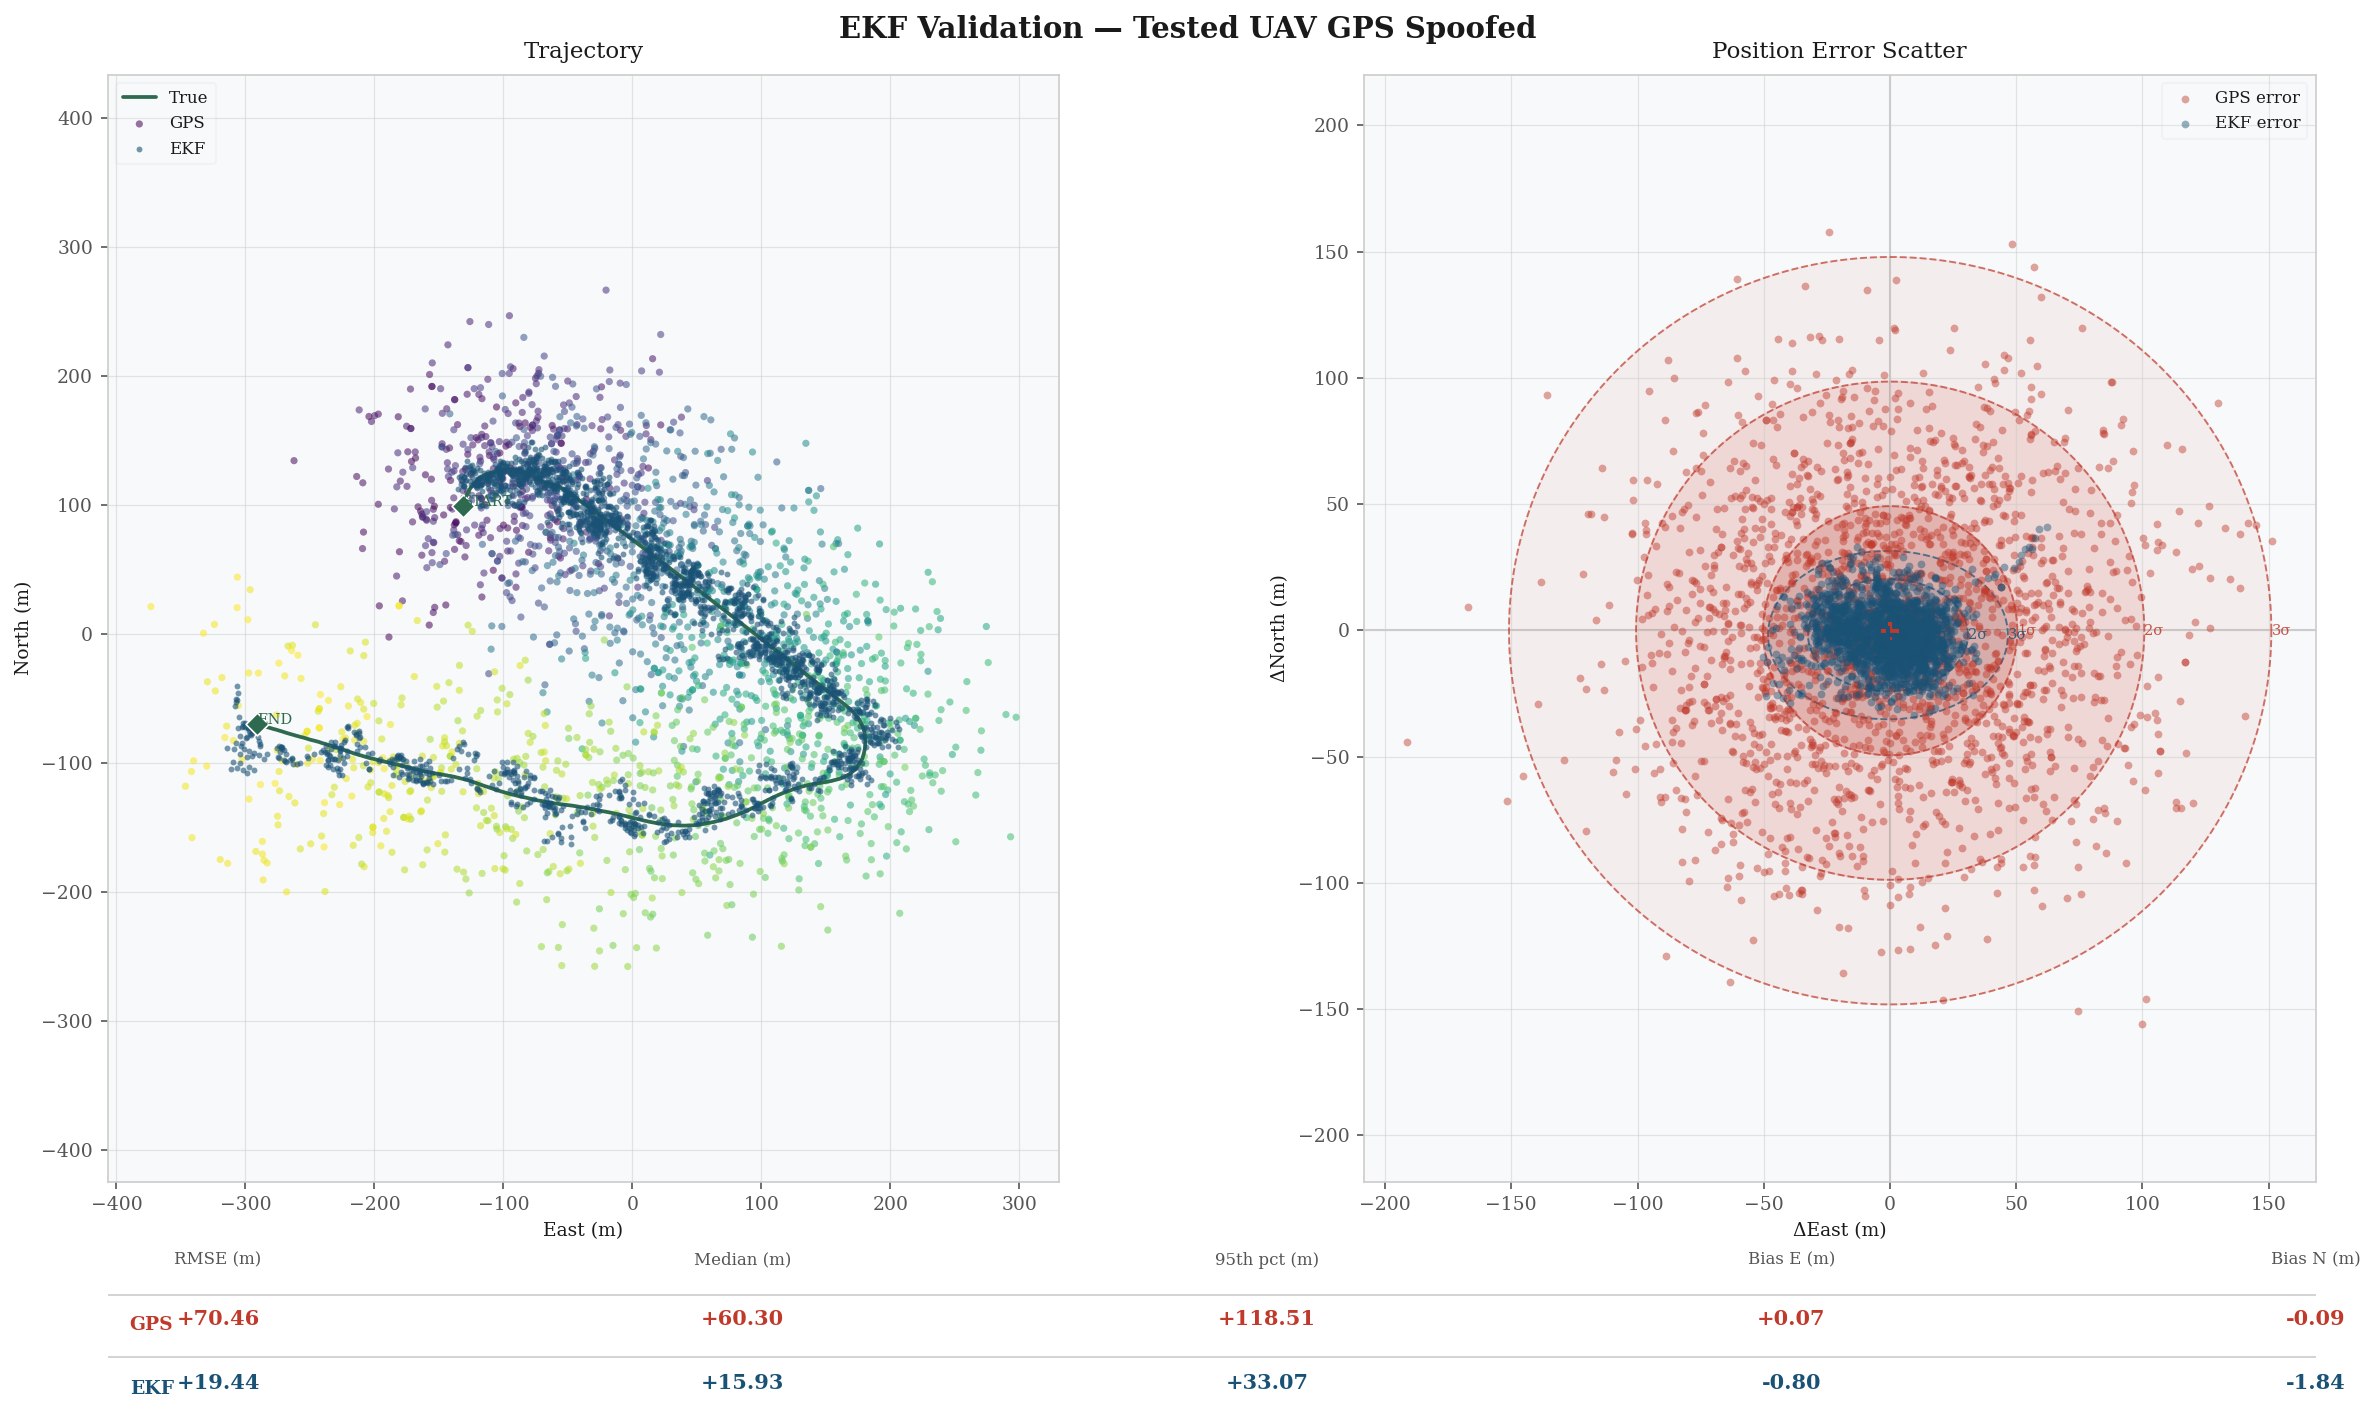
\includegraphics[width=0.9\textwidth]{images/ekf_validation_spoof_plot.png}
        \caption{KF test results for GPS spoofing. RED dots represent GPS position, BLUE dots represent KF position.}
        \label{fig:KF_test_gps_spoofing}
    \end{figure}



    Third test was ment to check if the KF is able to estimate the position of the drone even if half of the drones in the swarm are being spoofed. Again GPS was being spoofed with a random noise with a standard deviation of 70 meters. The results of the test are shown on the figure \ref{fig:KF_test_half_gps_spoofing}. As we can see, even if half of the drones in the swarm are being spoofed, KF is still able to estimate the position of the tested drone with a good accuracy, with RMSE around 1.6 meters, that is still better than the GPS alone, but not as good as in the normal operation.

    \begin{figure}[H]
        \centering
        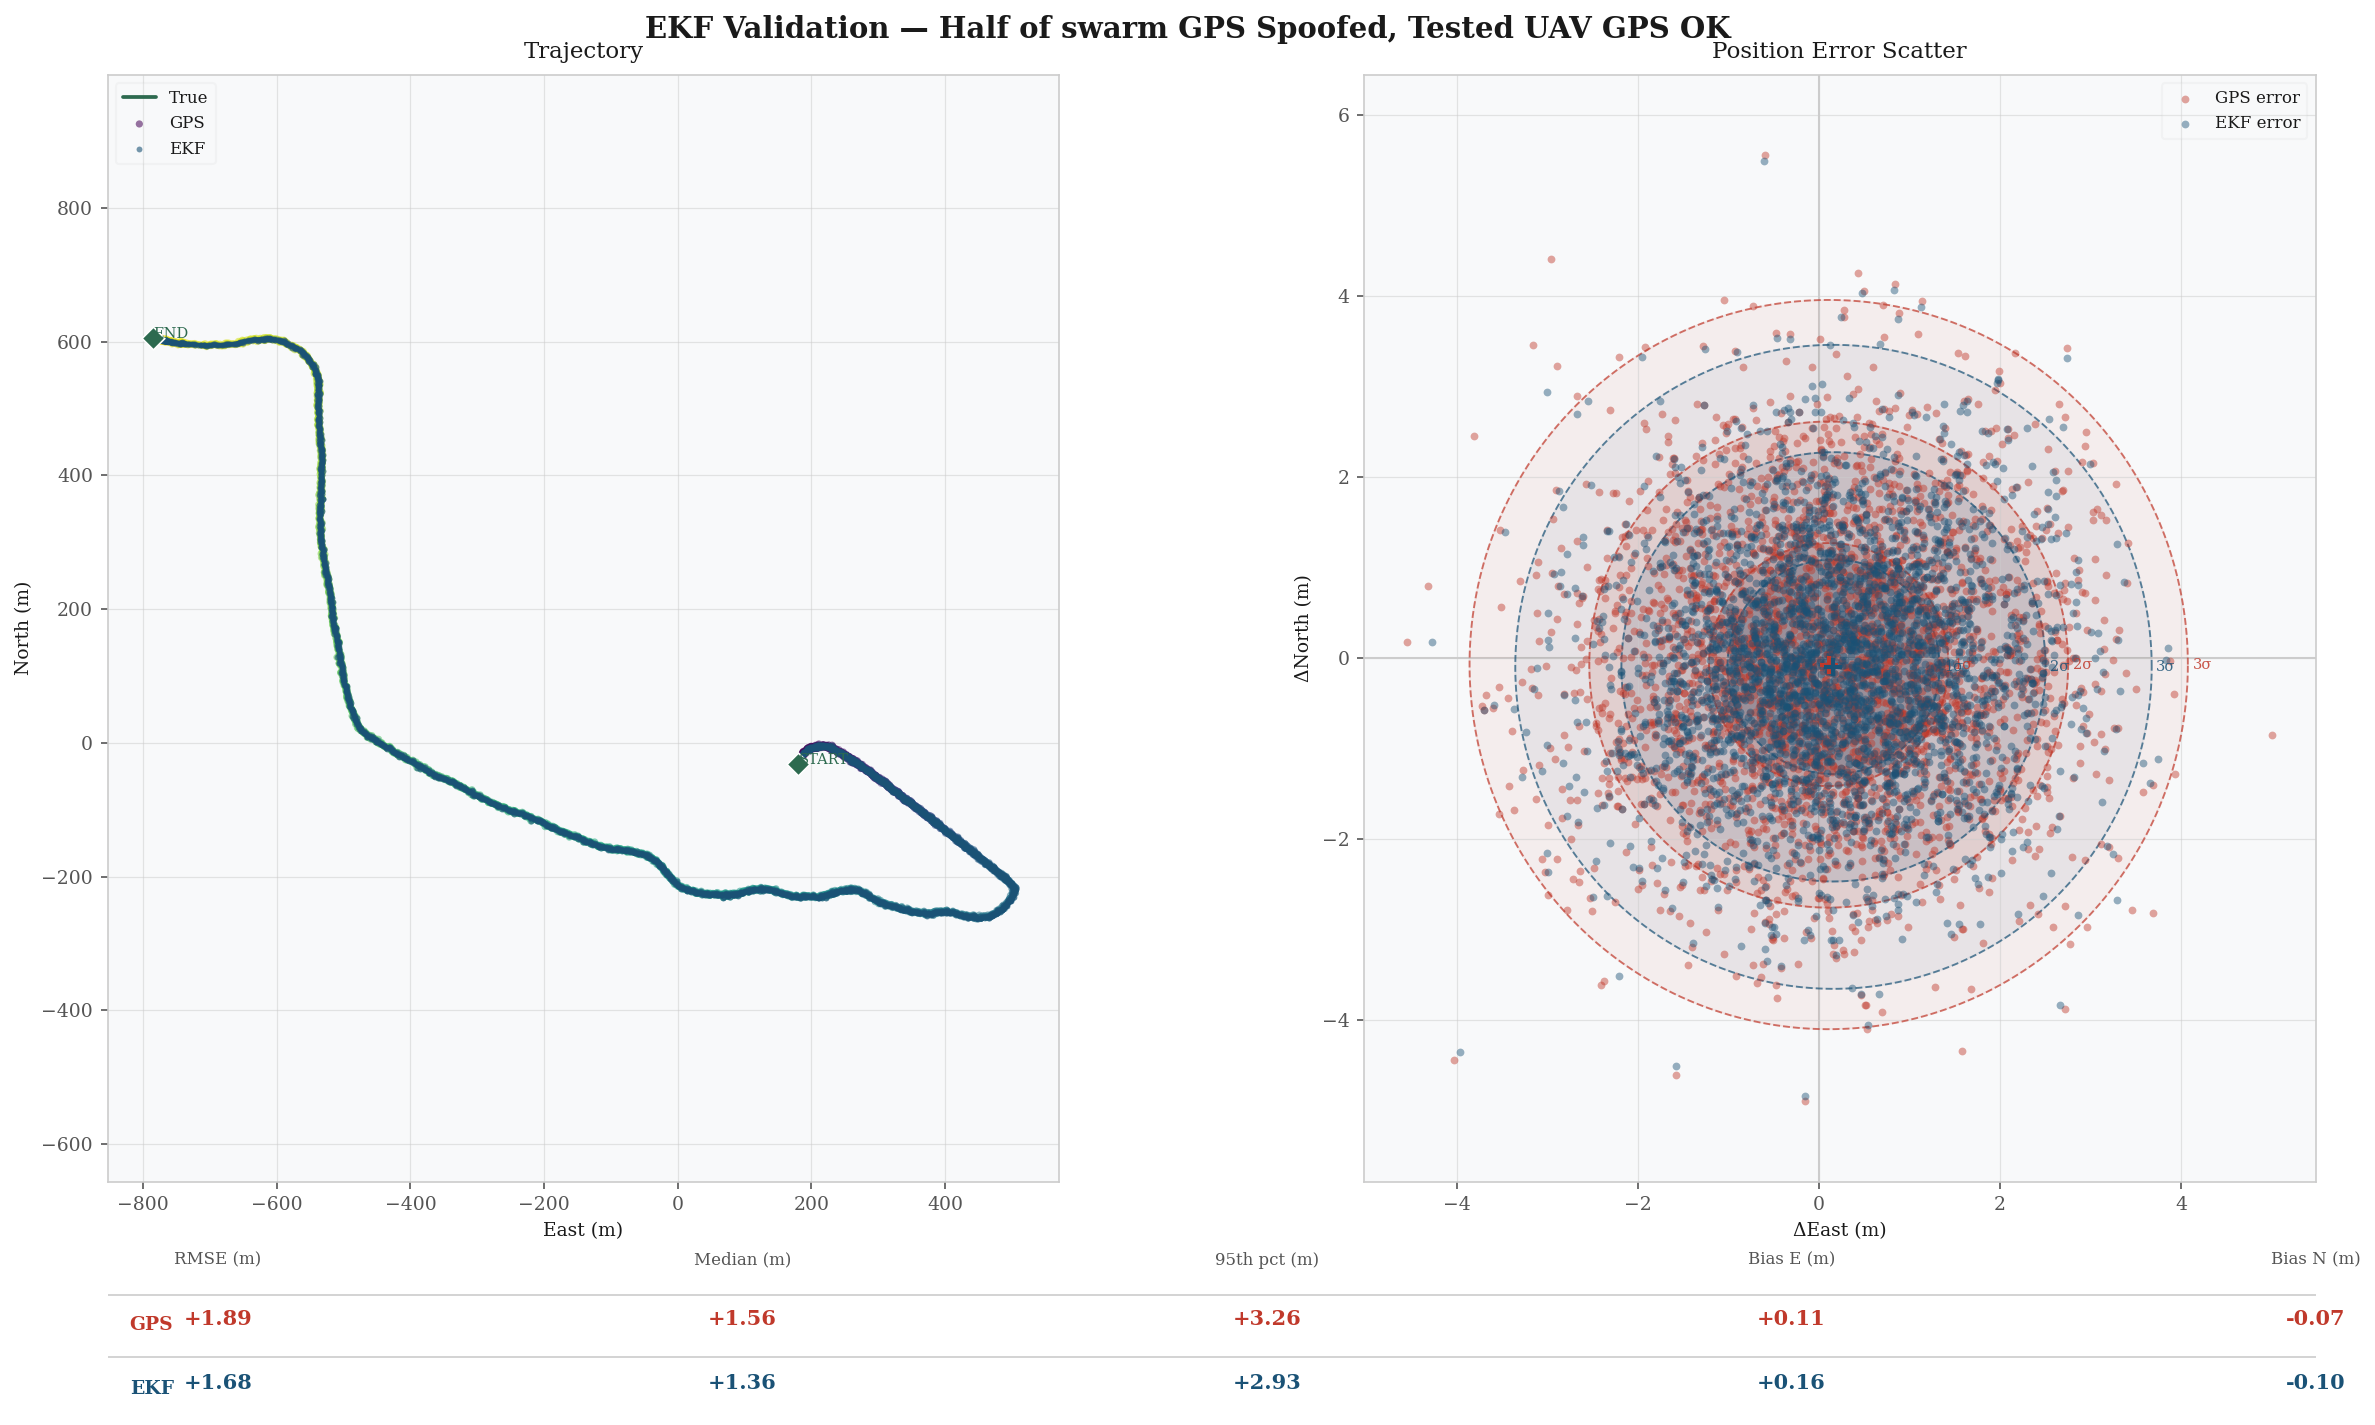
\includegraphics[width=0.9\textwidth]{images/ekf_validation_half_swarm_spoofed_plot.png}
        \caption{KF test results for half of the drones in the swarm being spoofed. RED dots represent GPS position, BLUE dots represent KF position.}
        \label{fig:KF_test_half_gps_spoofing}
    \end{figure}



\subsubsection{KF Validation Conclusion}

    Based on the results of the tests, I can conclude that the KF implementation is able to estimate the position of the drone with a good accuracy, even if one of the drones in the swarm is not able to receive GPS signal or if GPS signal is being spoofed. The KF is able to fuse data from multiple sensors and create a precise localization of drone in the swarm. In a future work it is possible to improve KF implementation by adding more sensors, such as camera or radar, to further improve the accuracy of the localization. Nevertheless, the current implementation is sufficient for the purpose of this project and is able to provide a good localization of drones in the swarm.

\subsection{Course and Speed Controller}

    As a course and speed controller I have implemented a simple PID controller that is able to keep the drone based on the desired course and speed. That kind of controller is not the most advanced one, but it is simple and effective for the purpose of this project. It is also possible to implement more advanced nonlinear controllers, such as INDI or ADRC ~\cite{wiki:adrc}, but that is out of the scope of this project. The main goal of this project is to create a simulator that is able to test swarm controllers, not to create the most advanced swarm controller. Nevertheless, the implemented PID controller is able to keep the drone on the desired course and speed with a good accuracy. 

    On a figure \ref{fig:PID_course_controller} is shown the response of the PID controller to a change in the desired course. As we can see, the drones are reaching a waypoint in a given distance and then changing the course to the next one.

    \begin{figure}[htbp]
        \centering
        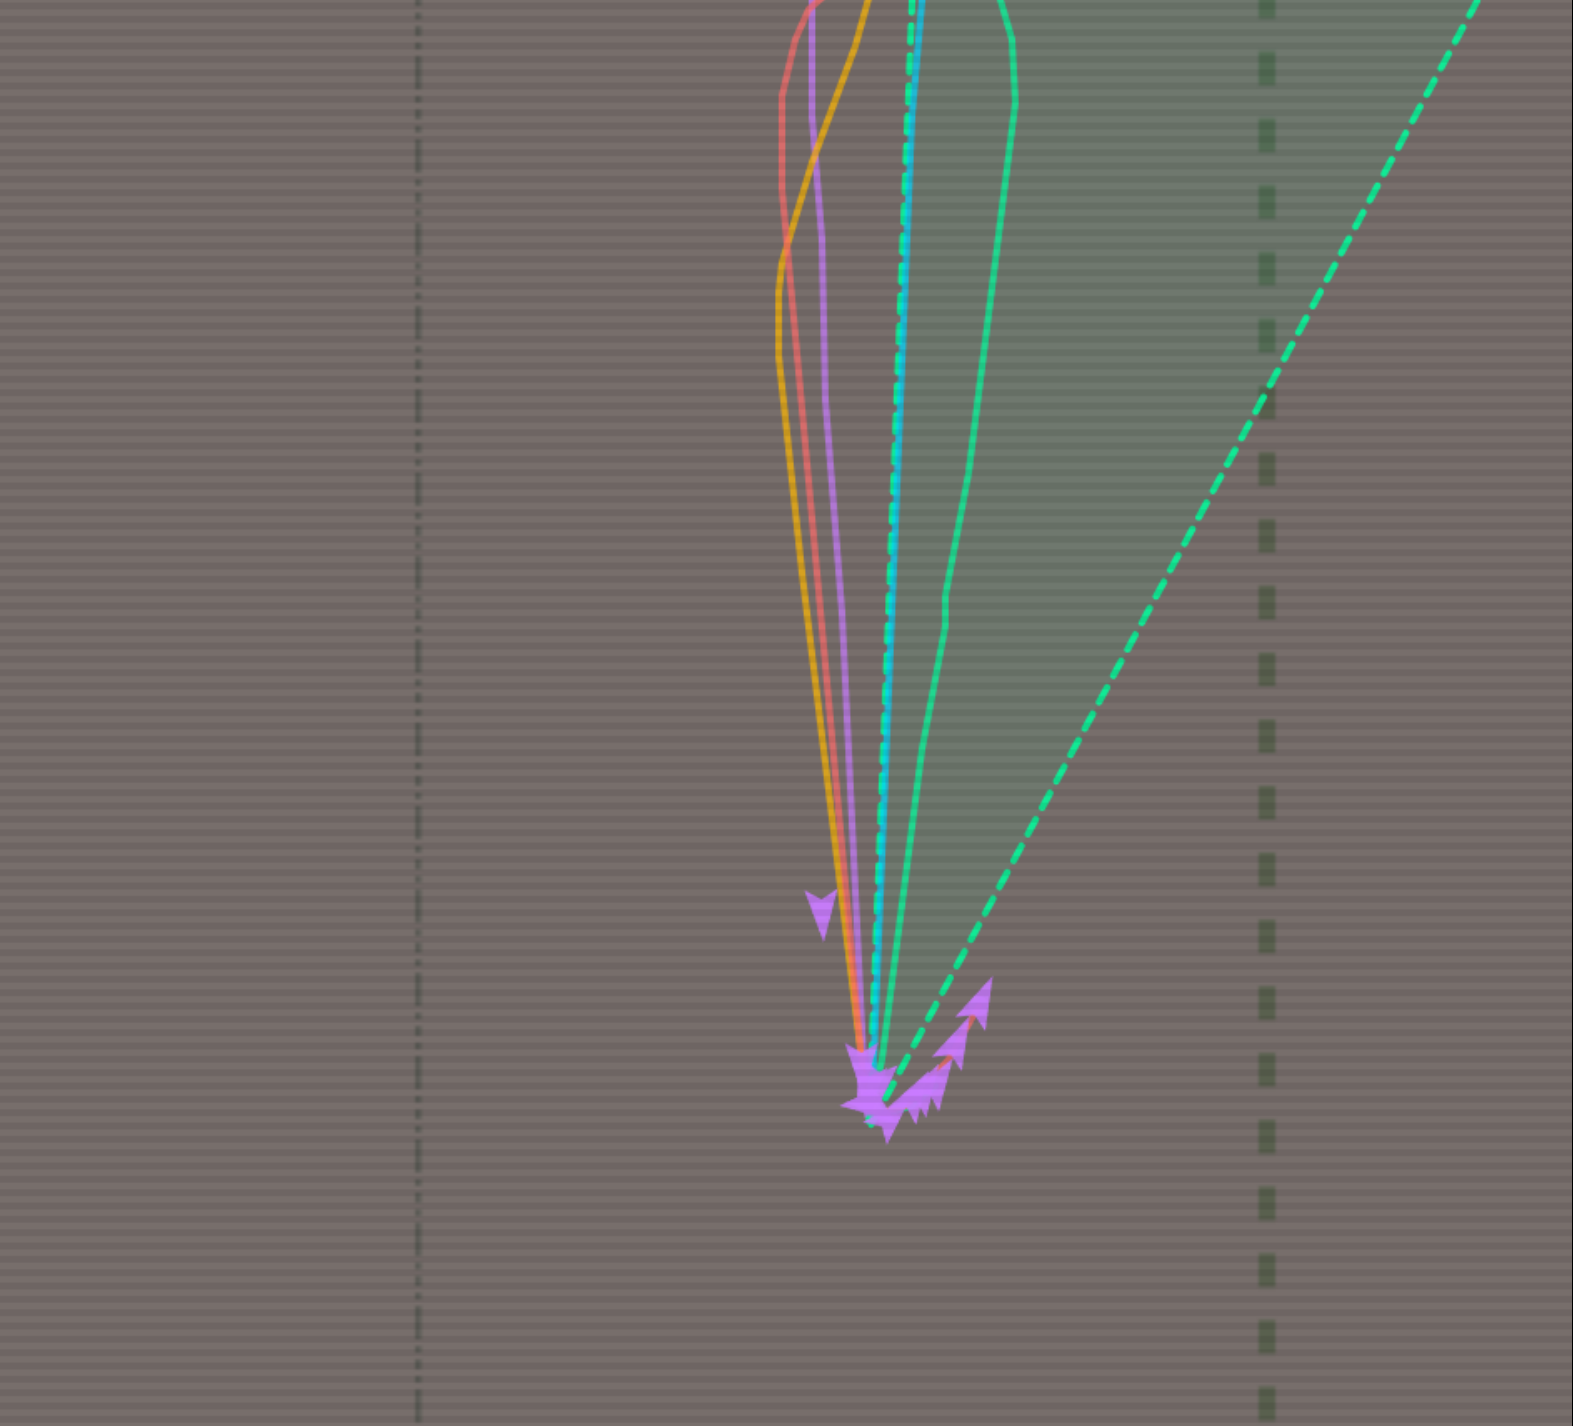
\includegraphics[width=0.7\textwidth]{images/PID_course_controller.png}
        \caption{PID controller keeping a course of a drone on the desired course. [UAV anti collision system not enabled!]}
        \label{fig:PID_course_controller}
    \end{figure}


\subsection{UAV Anti Collision System}

    In a drone swarms it is necessary to have an anti collison system. One avoiding collisons between drones in the swarm and a second one avoiding collisons with other vessels in the area. For now I will focus on the first one, avoiding collisons between drones in the swarm. 

    The system I have implemented is inspired by Newton's law of universal gravitation~\cite{newton1687principia}, which describes the electrostatic force between two charged particles. In this case, we can treat each drone as a charged particle and the force between them as a repulsive force that is proportional to the square of the distance between them. This means that the closer the drones are to each other, the stronger the repulsive force will be, which will help to avoid collisions between them.



    Whole system can be described by the following equation:


\begin{equation}
    \mathbf{F}_{ij} = 
    \begin{cases} 
        \frac{K}{d^2} \cdot \left( 1 - \frac{d}{d_{cut}} \right)^2 \cdot \frac{\mathbf{r}_{ij}}{d} & \text{for } d < d_{cut} \\ 
        0 & \text{for } d \geq d_{cut} 
    \end{cases}
\end{equation}

Where:
\begin{itemize}
    \item $K$ -- coefficient of repulsion (80000.f),
    \item $d_{cut}$ -- cutoff distance (200.f),
    \item $\frac{\mathbf{r}_{ij}}{d}$ -- unit vector of the force direction.
\end{itemize}


The total repulsive force acting on a drone $i$ is the vector sum of the forces from all other drones in the swarm:

\begin{equation}
\mathbf{F}_{total} = \sum_{j \neq i} \mathbf{F}_{ij} = \begin{bmatrix} F_x \\ F_z 
\end{bmatrix}
\end{equation}

In the end this force is used to alter the desired course of the drone to steer it away from the other drones in the swarm. The course alteration is calculated as follows:

\begin{equation}
    \psi_{rep} = \operatorname{atan2}(F_x, F_z)
\end{equation}

\begin{equation}
    \Delta\psi_{raw} = \operatorname{wrap}(\psi_{rep} - \psi_{curr})
\end{equation}


The final correction $\Delta\psi$ is scaled by the force magnitude and clamped to a predefined maximum range:
\begin{equation}
    \Delta\psi = \operatorname{clamp}\left( \Delta\psi_{raw} \cdot \frac{|\mathbf{F}{total}|}{100}, -\psi{max}, \psi_{max} \right)
\end{equation}


The speed reduction factor $v_{factor}$ depends linearly on the magnitude of the applied heading correction. This mechanism allows the unit to automatically decelerate while performing sharp evasive maneuvers:

\begin{equation}
    v_{factor} = 1 - \cdot \frac{|\Delta\psi|}{\psi_{max}}
\end{equation}


Theoretical way of operation is shown on the figure \ref{fig:collision_avoidance}.

\begin{figure}[htbp]
    \centering
    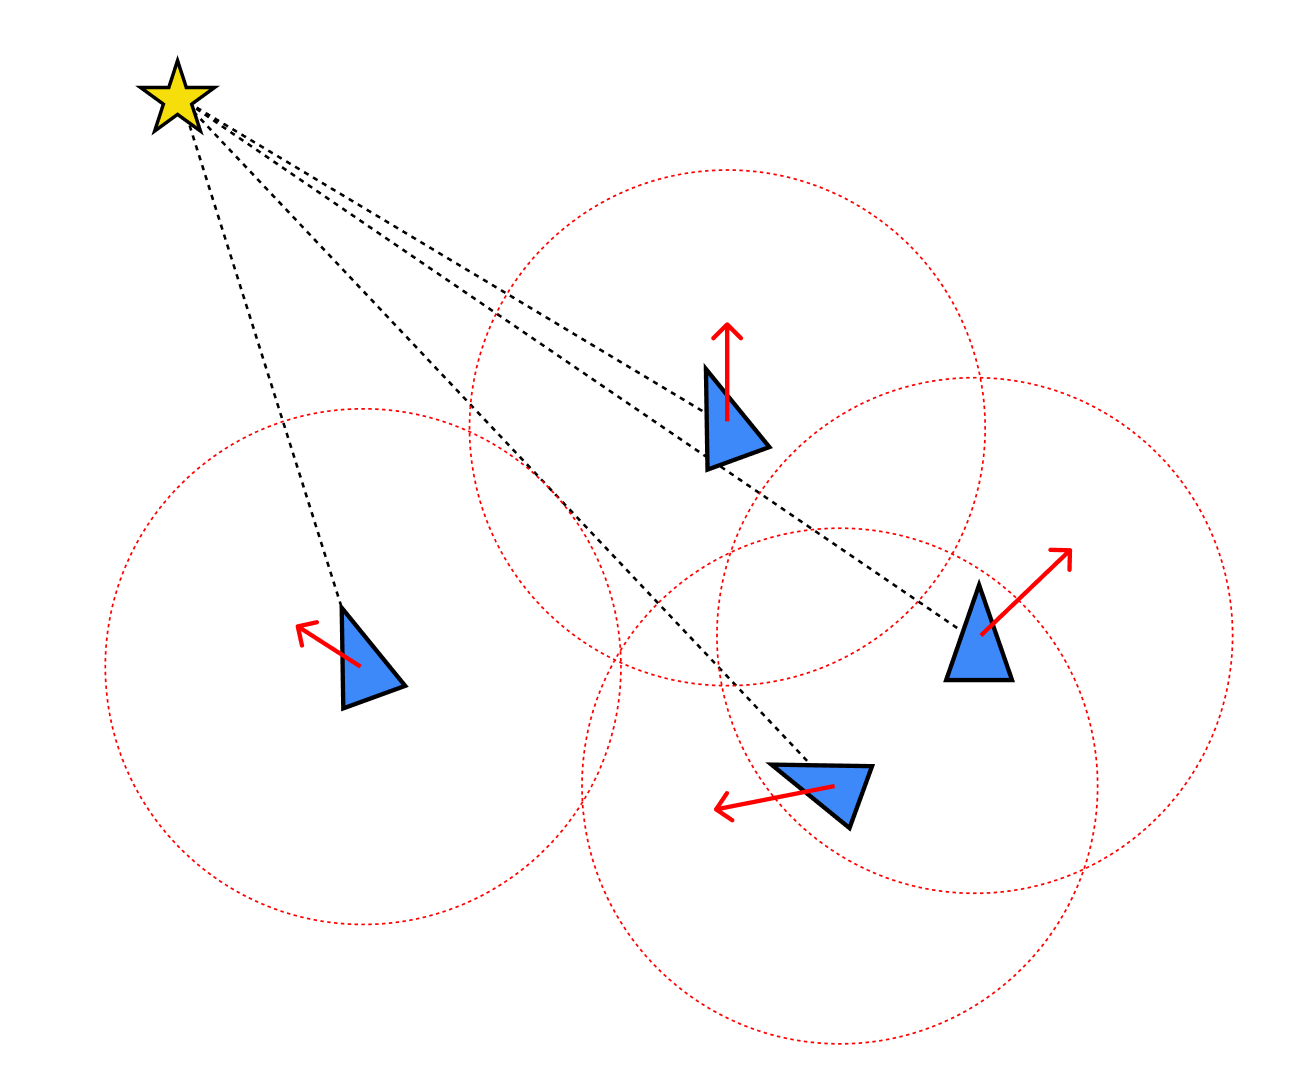
\includegraphics[width=0.5\textwidth]{images/anti_collison_graph_2.png}
    \caption{Collision avoidance system for a drone swarm. Star represents a drones goal position, red arrows represent the repulsive forces from other drones in the swarm, red dashed circle represents the effective repulsion force distance.}
    \label{fig:collision_avoidance}
\end{figure}


Algorithm tested in a simulator is able to keep the drones in the swarm away from each other and avoid collisions between them. It is very effective in preventing collisions.
On a figure \ref{fig:PID_course_controller} anti collision system is not active, so the drones are colliding with each other, on a way to waypoint.



\begin{figure}[htbp]
    \centering
    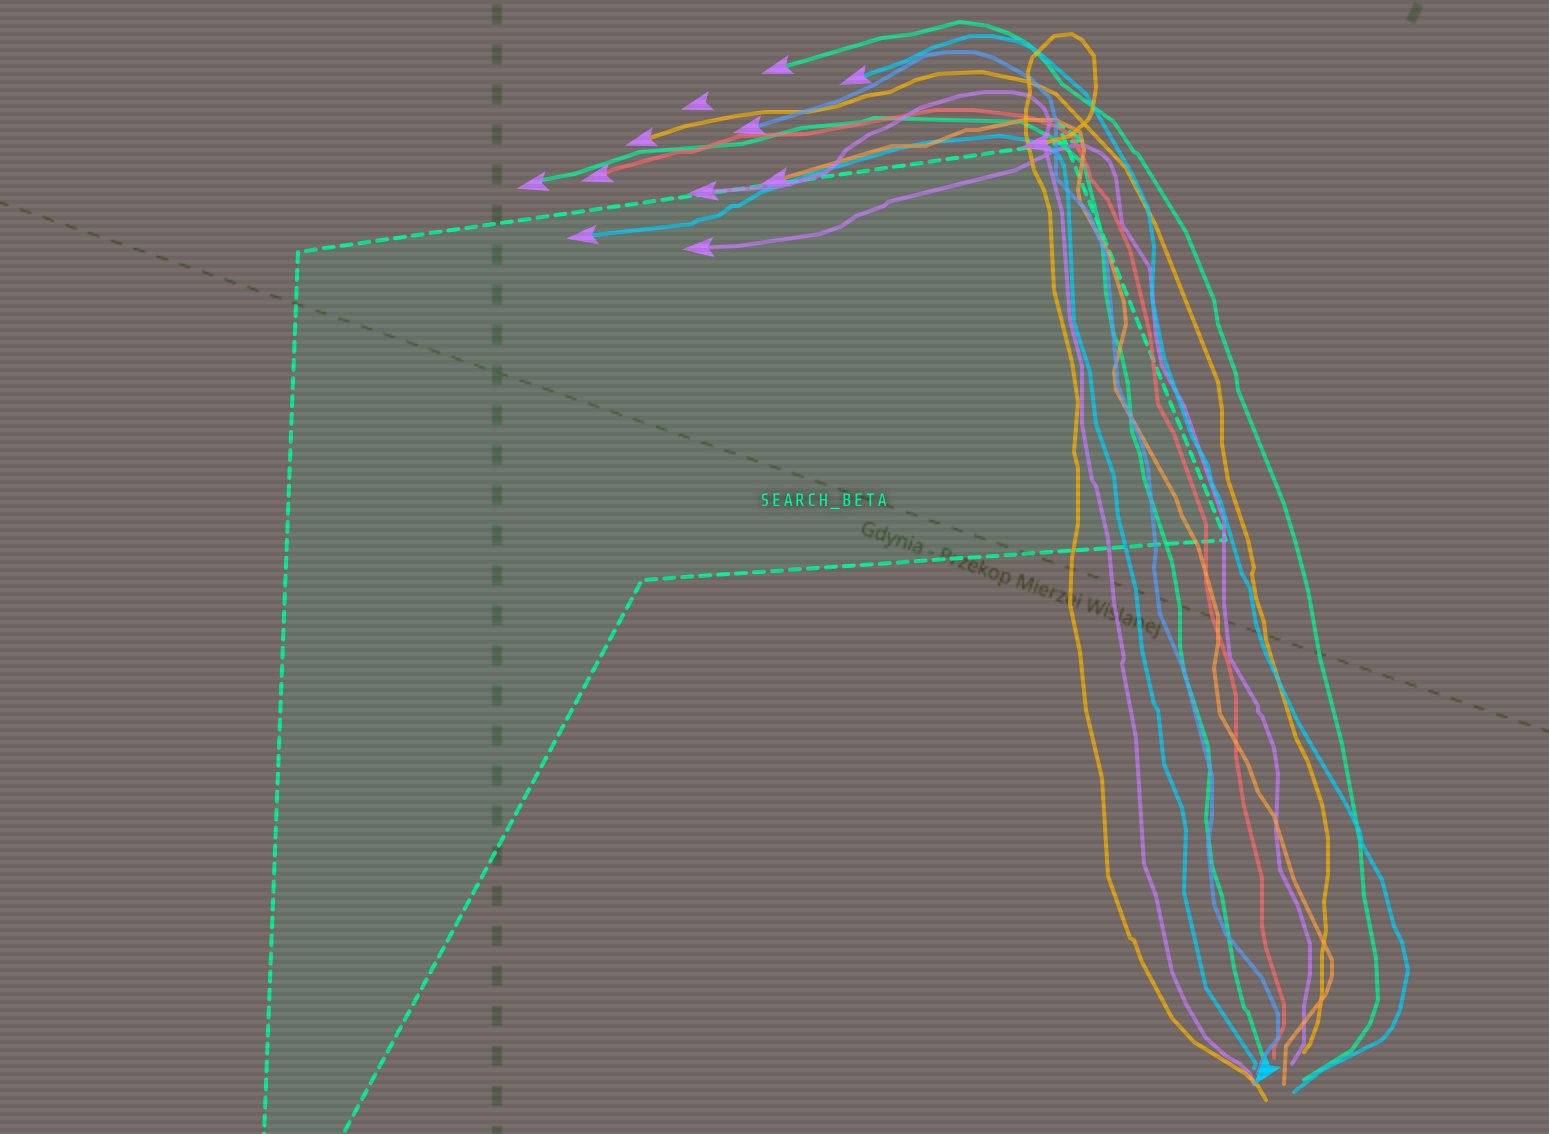
\includegraphics[width=0.8\textwidth]{images/UAV_collision_avoidance_test.png}
    \caption{Simulation of the collision avoidance system in action. System is especially effective when drones are in a close proximity to a waypoint. Yellow drone even have a circle manouver to avoid collison with other drones. The repulsive force is very well visible in the begining of drone path, when drones are in a close proximity to each other.}
    \label{fig:collision_avoidance_simulation}
\end{figure}





\subsection{AIS Vessels Avoidance System}

    The second part of the anti collison system is avoiding collisons with other vessels in the area, which are transmitting AIS signals. For that purpose I have implemented a simple system that is able to keep the drones away from the vessels in the area. The system is based on the same principle as the one for avoiding collisons between drones. The only difference is a reppeling force is not equal in all directions, but the shape of the force field is eliptical. This is because the drones are more likely to crash to big ship while being on its course rather than being on its side. 





\vspace{1cm}
\subsubsection{Elliptical Safety Zone (Mahalanobis Distance)}
Instead of a simple circle, the system defines a safety buffer around each ship. This buffer is stretched along the ship's heading to account for its momentum and restricted maneuverability. While creating this system I was inspired by Mahalanobis Distance, which is a measure of distance that accounts for the correlation between variables. In this case, eliptical safety zone is defined by ship lenght and speed. If the ship is stationary, the safety zone is a circle with a radius equal to the base radius determined by the vessel type. 


To determine the level of threat, the system calculates a normalized distance $d_{Maha}$. A value of $d_{Maha} < 1$ indicates that the drone has penetrated the safety buffer. The buffer is stretched along the ship's longitudinal axis to account for the vessel's momentum and limited maneuverability.

\begin{equation}
    d_{Maha} = \sqrt{ \left( \frac{x_{along}}{s_{along}} \right)^2 + \left( \frac{x_{perp}}{s_{perp}} \right)^2 }
\end{equation}

The scaling factors $s_{along}$ and $s_{perp}$ define the boundary of the ellipse:

\begin{itemize}
    \item $s_{perp} = R_{base}$ (The base radius determined by the vessel type).\item $s_{along} = 
    \begin{cases} R_{base} \cdot (1 + \sigma \cdot v_{ship}) & \text{if drone is ahead} \\ R_{base} \cdot \beta & \text{if drone is behind} \end{cases}$
\end{itemize}

Where:
\begin{itemize}
    \item $\sigma$ -- Speed stretch factor = 0.2.
    \item $\beta$ -- Behind factor = 0.4.
    \item $v_{ship}$ -- Velocity of the vessel in m/s.
\end{itemize}



\vspace{1cm}
If the drone enters the safety zone, the system calculates an Escape Bearing $\psi_{esc}$. The strategy commands the drone to steer perpendicular to the ship's track, choosing the side that minimizes the time spent within the danger area:

\begin{equation}
    \psi_{esc} = 
    \begin{cases} 
        \psi_{ship} - 90^\circ & \text{if } x_{perp} \geq 0 \\ 
        \psi_{ship} + 90^\circ & \text{if } x_{perp} < 0 
    \end{cases}
\end{equation}


The final control output is determined by the severity of the intrusion. In the DANGER zone, the navigation logic is entirely bypassed in favor of maximum evasive maneuvers:

\begin{equation}
\text{Final Command} =
\begin{cases}
    \text{Steer}_{\max}, \text{Thr}_{\min} & \text{if } d_{Maha} < Z_{\text{danger}} \\
    \text{Interpolated Transition} & \text{if } Z_{\text{danger}} \leq d_{Maha} < Z_{\text{warning}} \\
    \text{Standard Navigation} & \text{if } d_{Maha} \geq 1
\end{cases}
\end{equation}


\vspace{0.5cm}

\begin{figure}[htbp]
    \centering
    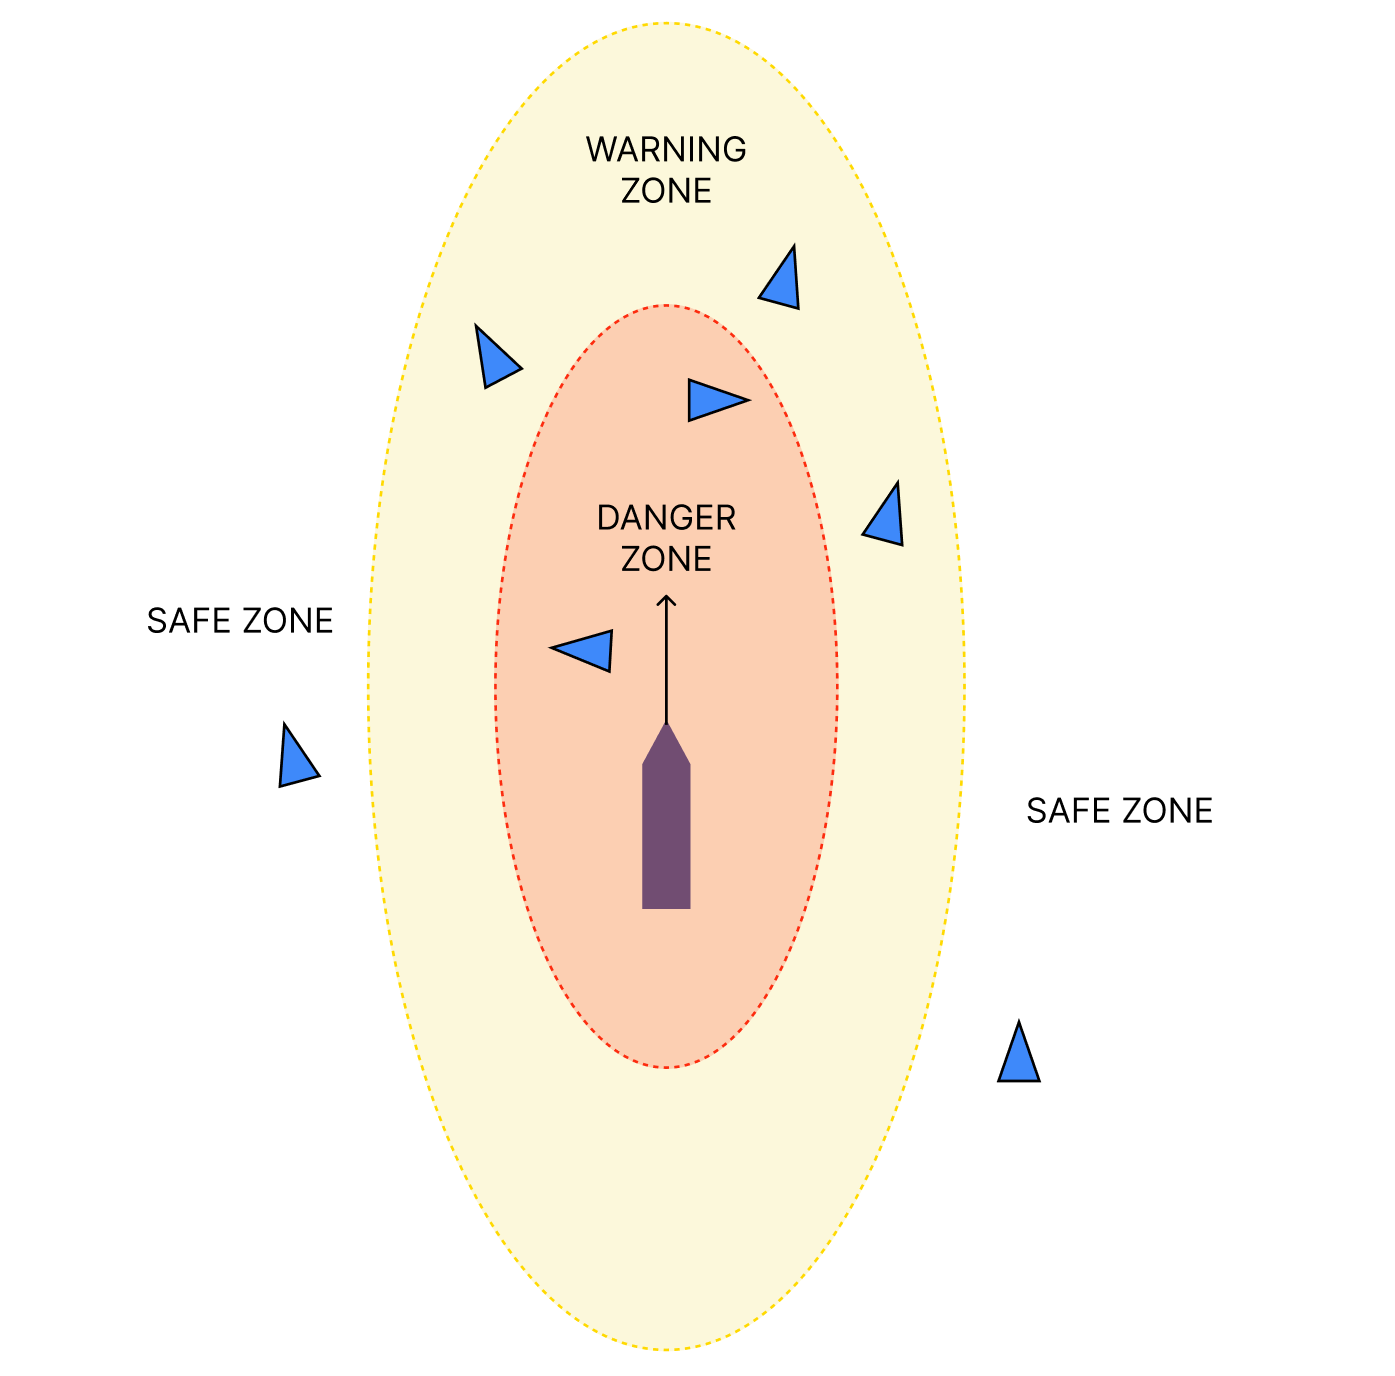
\includegraphics[width=0.65\textwidth]{images/safety_zone2.png}
    \caption{Elliptical safety zone around a large vessel. Blue arrows represents UAVS, puprle arrow represents a big ship. The safety zone is stretched and shifted along the ship's heading to account for its momentum.}
    \label{fig:big_ship_safe_zone}
\end{figure}




\begin{figure}[htbp]
    \centering
    \begin{subfigure}{0.48\textwidth}
        \centering
        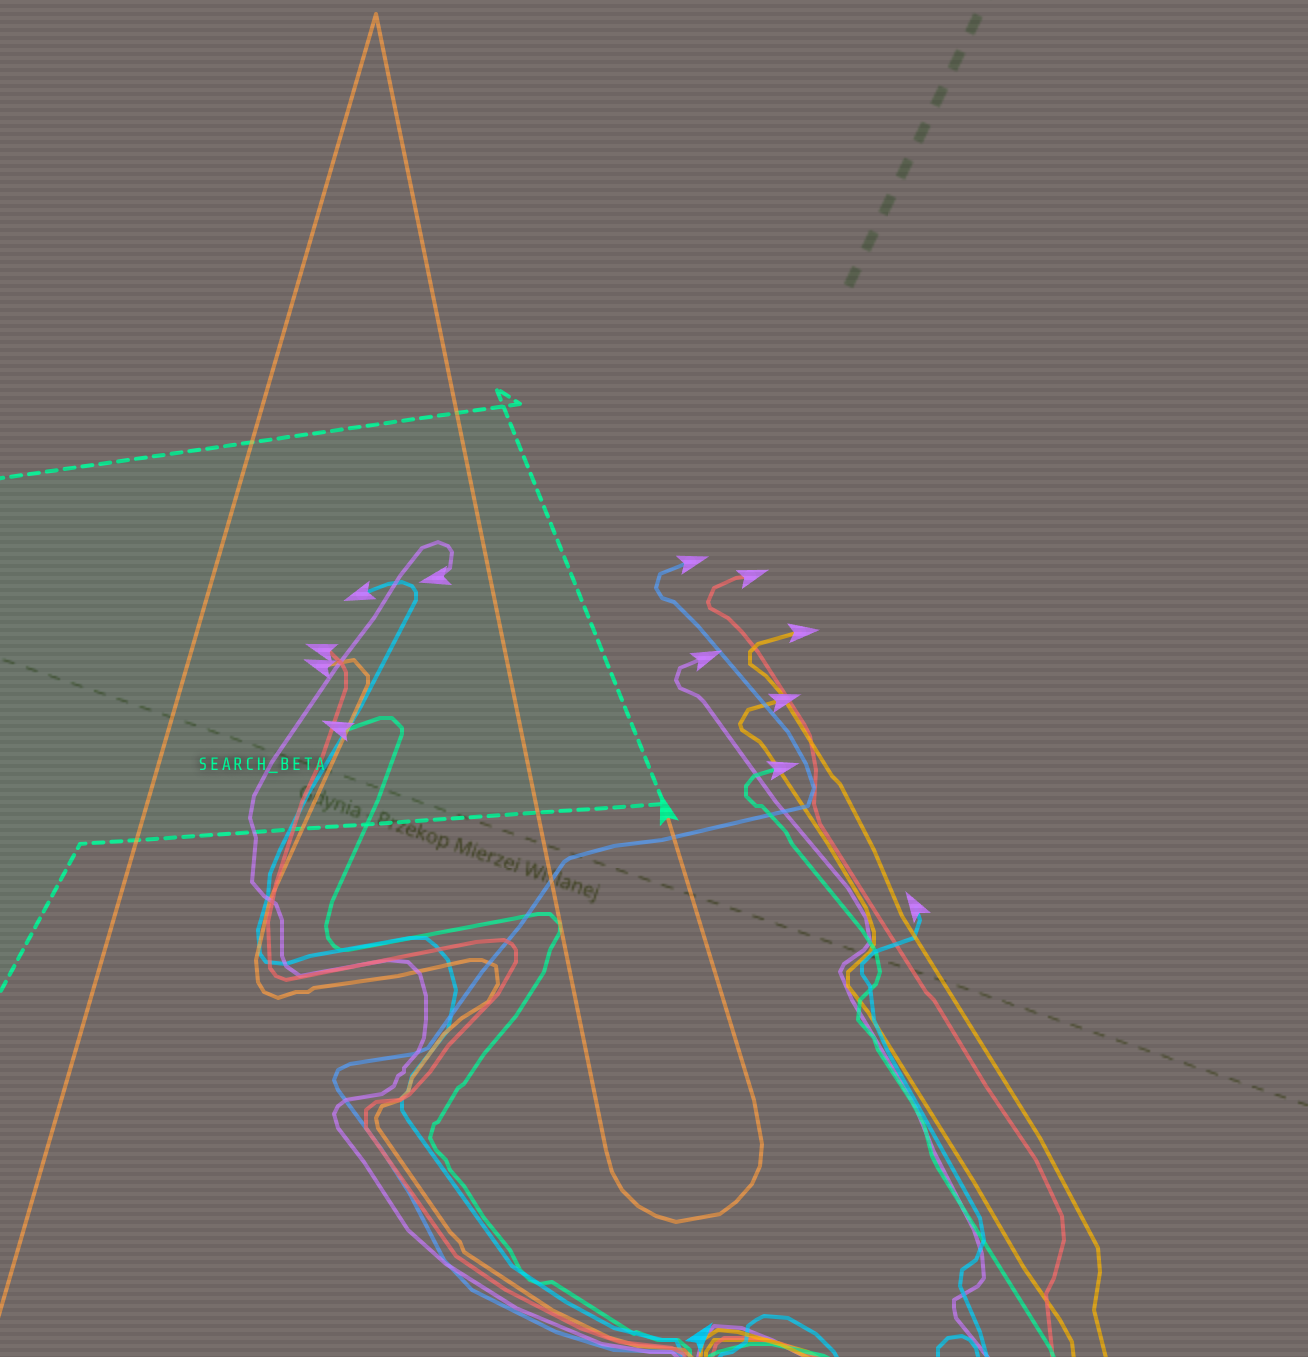
\includegraphics[width=\textwidth]{images/ais_avoidance_test_01.png}
        \caption{Initial approach: The vessel (yellow) approaches at 35\,kts. Drones are initially on a collision course. Drones immediately detect the vessel and begin evasive maneuvers to steer clear of the safety zone.}
        \label{fig:big_ship_avoidance_simulation_1}
    \end{subfigure}
    \hfill
    \begin{subfigure}{0.48\textwidth}
        \centering
        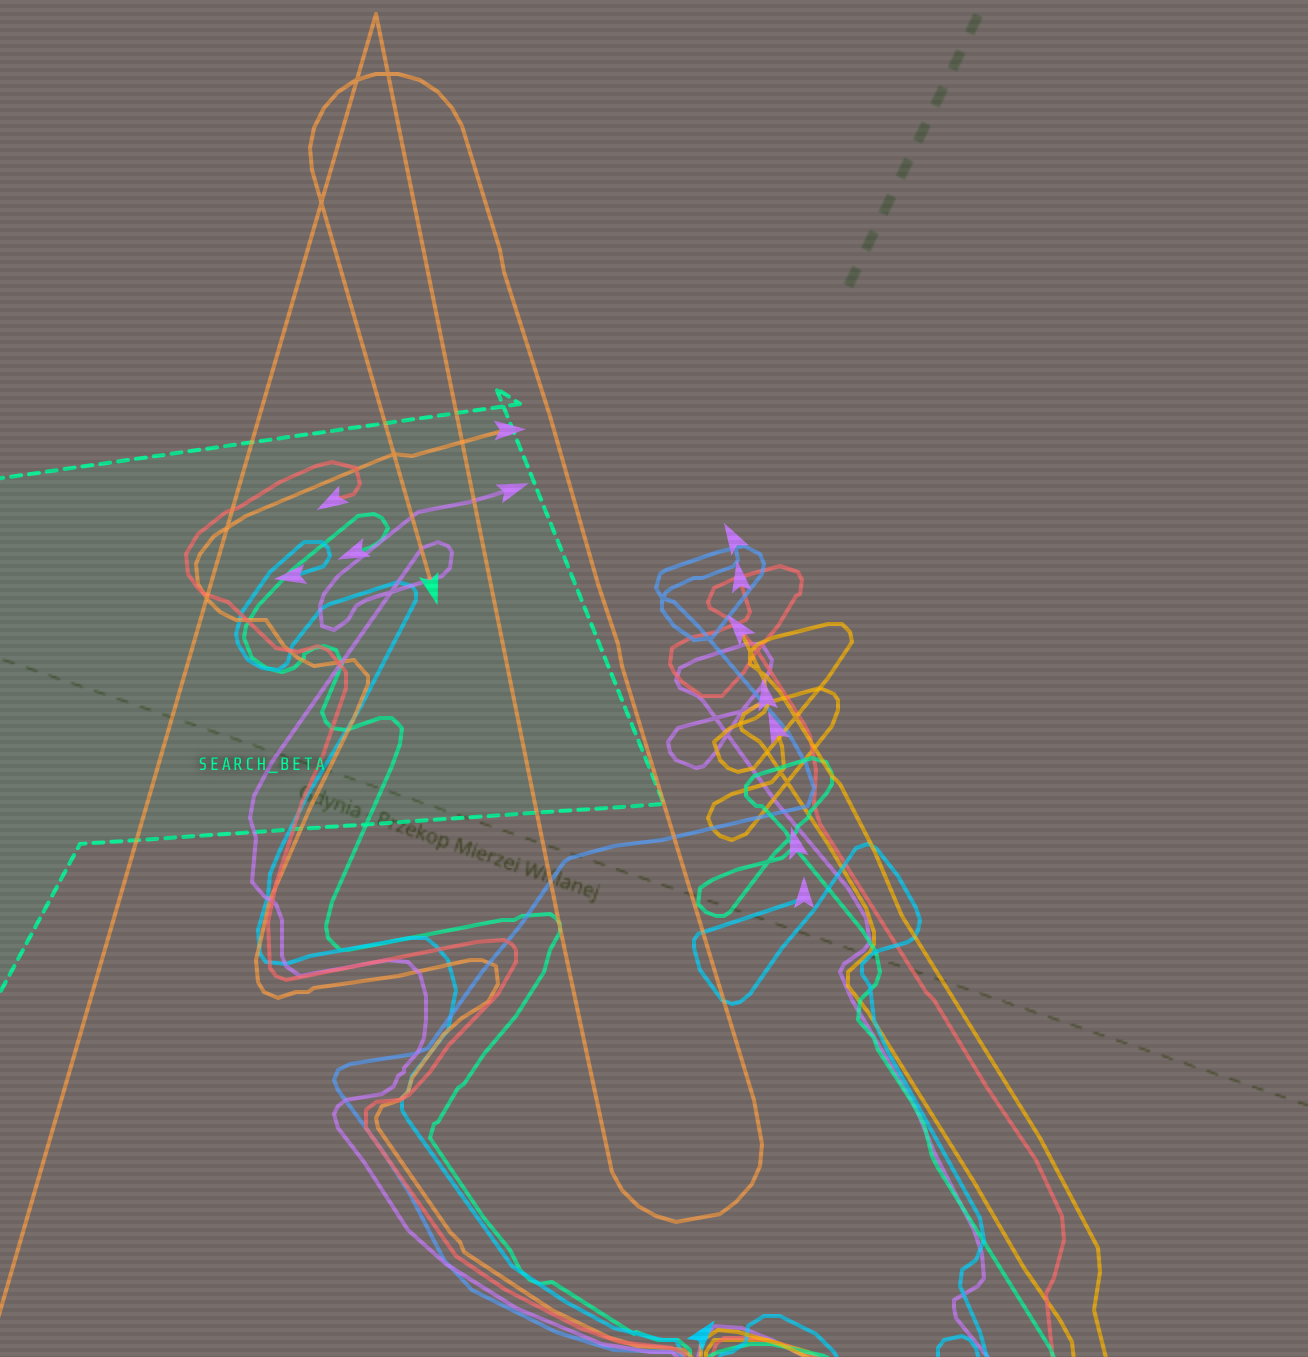
\includegraphics[width=\textwidth]{images/ais_avoidance_test_02.png}
        \caption{Continous avoidance: Yellow ship makes sharp U turn going back into drones trajectory. UAVs deviate from the ship's trajectory to minimize time in the danger zone, and tries to achieve a waypoint at a same time.}
        \label{fig:big_ship_avoidance_simulation_2}
    \end{subfigure}

    \caption{Simulation of the AIS vessel avoidance system. The drones successfully detect and maneuver around the high-speed commercial vessel to maintain the safety buffer, while still progressing towards their waypoint. The elliptical safety zone is clearly visible as the drones adjust their paths to minimize time spent within it.}
    \label{fig:big_ship_avoidance_simulation}
\end{figure}




\vspace{1cm}
\subsubsection{Potential Problems}
    The major problem of this system is assumption that all vessels in the area are transmitting AIS signals. In reality, there are many vessels that are not, either because they are not required to do so or because they are intentionally trying to avoid detection. Other issue is a position of the vessel is taken from onboard GPS, which can be easily spoofed or jammed. In that case, the system will not be able to detect the vessel and avoid collison with it. That is why it is important to have a backup system that is able to detect vessels in the area even if they are not transmitting AIS signals. One possible solution is to use radar or camera to detect vessels in the area and avoid collison with them. That is out of the scope of this project, but it is something that could be implemented in the future.

